\documentclass[openany]{book}
\input{notes_white}
\usepackage{mathtools}
\usepackage{pgfplots}
\settitle{Biology Lab Manual - Expt 3}
\begin{document}
\title{\Large{\underemphasise{Biology - Expt 3}} \\ \vspace{5pt}
\large{Determining Column Dead Volume– Gel Filtration Chromatography}}
\author{Eklavya Raman \\ \vspace{5pt} er24ms024@iiserkol.ac.in \\ \vspace{5pt}}
\date{\today}
\maketitle
\begin{center}
    \textbf{Abstract}
\end{center}
    Gel filtration chromatography, also known as size-exclusion chromatography, is a technique used to separate molecules based on their size. This experiment aims to determine the column void volume ($V_0$) of a gel filtration column using standard proteins of known molecular weights. The void volume is the volume of mobile phase in the column that is not occupied by the stationary phase and is crucial for understanding the separation efficiency of the column. By analyzing the elution profiles of standard proteins, we can calculate $V_0$ and assess the performance of the gel filtration column.
\subsubsection{Aim}
To separate molecules based on their size using gel filtration chromatography (size exclusion chromatography) and to determine the void volume ($V_0$) of the column using Blue Dextran.
\subsubsection{Apparatus}
\begin{itemize}
    \item Gel Filtration Column (Sephadex G-25)
    \item Blue Dextran as standard protein
    \item Buffer Solution (e.g., Phosphate Buffered Saline)
    \item UV-Vis Spectrophotometer
    \item Fraction Collector or Test Tubes
    \item Pipettes and Micropipettes
\end{itemize}
\subsubsection{Working Principle and Formula}
Gel filtration chromatography separates molecules based on their size as they pass through a column packed with porous beads. Larger molecules are excluded from entering the pores and thus elute first, while smaller molecules enter the pores and elute later. The void volume ($V_0$) is the volume of mobile phase in the column that is not occupied by the stationary phase (the beads). It can be determined using a standard molecule that is too large to enter the pores, such as Blue Dextran. We measure the elution volume ($V_e$) of Blue Dextran, which corresponds to the void volume ($V_0$). The formula to calculate the void volume is:
$$V_0 = V_e$$
To measure the elution volume, we collect fractions of the eluent and measure their absorbance at a specific wavelength (e.g., 280 nm for proteins) using a UV-Vis spectrophotometer. The elution profile is plotted as absorbance versus fraction number, and the peak corresponding to Blue Dextran indicates the void volume.
The void volume is given by the formula: 
$$\boxed{V_0 = \text{Initial Volume of Buffer} + (n \times (0.5))}$$
where $n$ is the number of fractions collected before the peak of Blue Dextran.
\subsubsection{Experimental Procedure}
\begin{enumerate}
    \item Prepare the gel filtration column by equilibrating it with the buffer solution.
    \item Ensure there are no air bubbles in the column and that gel is properly packed.
    \item Load a known volume (e.g., 1 mL) of Blue Dextran solution onto the top of the column.
    \item Allow the sample to enter the gel bed by gravity flow or gentle pressure.
    \item Elute the column with the buffer solution, collecting fractions (10 mL each) in test tubes or a fraction collector.
    \item Measure the absorbance of each fraction at 280 nm using a UV-Vis spectrophotometer.
    \item Plot the absorbance against fraction number to obtain the elution profile.
    \item Identify the peak corresponding to Blue Dextran and determine the elution volume ($V_e$).
    \item Measure the initial volume of buffer used and calculate the void volume ($V_0$) using the formula provided.
\end{enumerate}
\subsubsection{Observations and Results}
\textbf{Initial Volume of Buffer: } 7 mL \\
\textbf{Absorbance Data: } \\
\begin{figure}[H]
    \centering
    \begin{tabular}{|c|c|}
        \hline
        Fraction Number & Absorbance \\
        \hline
        1 & 0.206 \\
        2 & 0.892 \\
        3 & 1.650 \\
        4 & 1.732 \\
        5 & 1.617 \\
        6 & 1.504 \\
        7 & 1.255\\
        8 & 0.927 \\
        9 & 0.562 \\
        10 & 0.480 \\
        \hline
    \end{tabular}
    \captionof{table}{Absorbance Data for Blue Dextran Elution}
    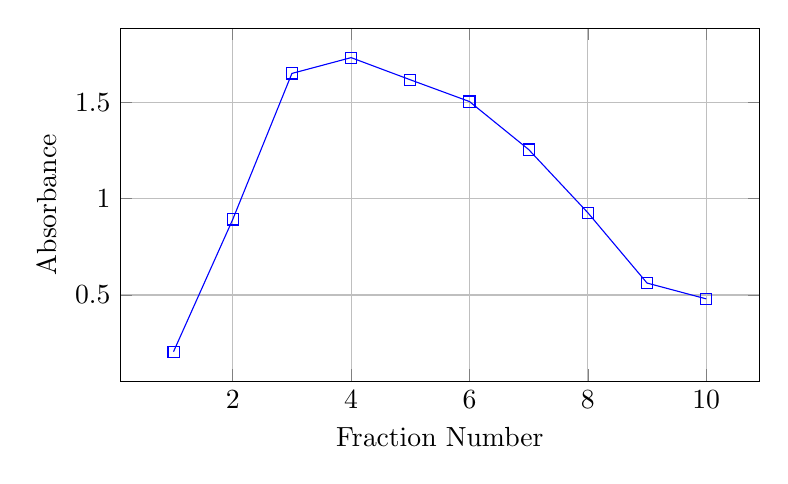
\begin{tikzpicture}
        \begin{axis}[
            xlabel={Fraction Number},
            ylabel={Absorbance},
            grid=major,
            width=0.8\textwidth,
            height=0.5\textwidth
        ]
        \addplot[
            color=blue,
            mark=square,
            ]
            coordinates {
            (1,0.206)(2,0.892)(3,1.650)(4,1.732)(5,1.617)(6,1.504)(7,1.255)(8,0.927)(9,0.562)(10,0.480)
            };
        \end{axis}
    \end{tikzpicture}
    \captionof{figure}{Number of fractions vs Absorbance}
\end{figure}
We have 
$n = 4$ (number of fractions before the peak of Blue Dextran) \\
$$V_0 = \text{Initial Volume of Buffer} + (n \times (0.5)) = \boxed{7 + (4 \times 0.5) = 7 + 2 = 9 \text{ mL}}$$
\subsubsection{Conclusion}
The void volume ($V_0$) of the gel filtration column was determined to be 9 mL using Blue Dextran as a standard. This value is essential for understanding the separation efficiency of the column and can be used in future experiments to analyze the size of unknown molecules. The experiment successfully demonstrated the principles of gel filtration chromatography and the calculation of void volume.

\end{document}